% Student template

\clearpage

\providecommand\studentimages[1]{%
	% Bild in Ring
	\begin{tikzpicture}[remember picture, overlay]
		\node[inner sep=0pt] at (2, -4) {
			\includegraphics[keepaspectratio=true, width=200pt]{parts/students/figures/#1.jpg}
		};
	\end{tikzpicture}

	% Ring
	\begin{tikzpicture}[remember picture, overlay]
		\node[inner sep=0pt] at (2, -4) {
			
\includegraphics[keepaspectratio=true, width=250pt]{ring.png}
		};
	\end{tikzpicture}

	% Bild in Rahmen
	\begin{tikzpicture}[remember picture, overlay]
		\node[inner sep=0pt] at (14, -18.5) {
			\includegraphics[keepaspectratio=true, width=160pt]{parts/students/figures/#1_child.jpg}
		};
	\end{tikzpicture}

	% Rahmen
	\begin{tikzpicture}[remember picture, overlay]
		\node[inner sep=0pt] at (14, -18) {
			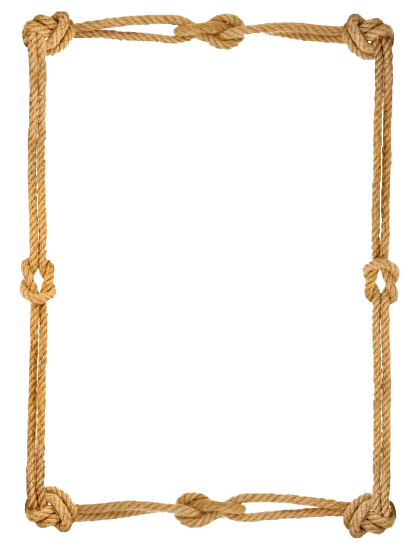
\includegraphics[keepaspectratio=true, width=180pt]{rahmen.png}
		};
	\end{tikzpicture}
}

\providecommand\studentprofile[8]{%
	\sectionmark{Steckbrief - #1}

	% Steckbrief Tabelle
	\begin{tikzpicture}[overlay]
		\node[text width=250pt, align=left] at (12, -4) {
			\Large{\begin{tabular}{@{}ll@{}}
				\textbf{Name:} & #1 \\
				\textbf{Geburtstag:} & #2 \\
				\textbf{Lieblingsfach:} & #3 \\
				\textbf{Hobbies:} & #4 \\
				\textbf{Lieblingsgenre:} & #5 \\
			\end{tabular}}\\~\\
			\textbf{Das werde ich am meisten vermissen:}\\#6\\~\\
			\textbf{Ohne das hätte ich die Oberstufe nicht geschafft:}\\#7\\~\\
			\textbf{Lebensmotto:}\\#8\\~\\
		};
	\end{tikzpicture}
}

\providecommand\studenttable[2]{%
	\vskip 9cm
	\hspace*{-1.2cm}
	\Large{\begin{tabular}{@{}ll@{}}
		\textbf{Erkennungsmerkmale:} & #1 \\
		\textbf{Zukunftspläne:} & #2 \\
	\end{tabular}}
}

\providecommand\studentcomments[1]{%
	\begin{figure}[H]
		\hspace*{-2.5cm}
\includegraphics[keepaspectratio=true, width=\paperwidth]{mittelwelle.png}
	\end{figure}
}
